
%(BEGIN_QUESTION)
% Copyright 2012, Tony R. Kuphaldt, released under the Creative Commons Attribution License (v 1.0)
% This means you may do almost anything with this work of mine, so long as you give me proper credit

A {\it centrifugal pump} works by spinning a disk with radial vanes called an ``impeller,'' which flings fluid outward from the center of the disk to the edge of the disk.  This kinetic energy imparted to the fluid translates to potential energy in the form of pressure when the fluid molecules strike the inner wall of the pump casing:

$$\includegraphics[width=15.5cm]{i02588x01.eps}$$

The energy conveyed by the liquid exiting the discharge port of this pump comes in two forms: {\it pressure head} and {\it velocity head}.  Ignoring differences in elevation (height), we may apply Bernoulli's equation to describe this fluid energy:

$$\hbox{Fluid Energy at discharge port} = {\rho v^2 \over 2} + P$$

\noindent
Where,

Fluid Energy = expressed in units of pounds per square foot, or PSF

$P$ = Gauge pressure (pounds per square foot, or PSF)

$\rho$ = Mass density of fluid (slugs per cubic foot)

$v$ = Velocity of fluid (feet per second)

\vskip 10pt

When the discharge port is completely blocked by an obstruction such as a closed valve or a blind, there is no velocity at the port ($v = 0$) and therefore the total energy is in the potential form of pressure ($P$).  When the discharge port is completely unobstructed, there will be no pressure at the port ($P = 0$) and therefore the total energy is in kinetic form (${\rho v^2 \over 2}$).  During normal operation when the discharge experiences some degree of resistance, the discharge fluid stream will possess some velocity as well as some pressure.

\vskip 10pt

Assuming that the fluid molecules' maximum velocity is equal to the speed of the impeller's rim, calculate the discharge pressure under these conditions for a pump having an 8 inch diameter impeller spinning at 1760 RPM and a discharge port of 2 inches diameter, with water as the fluid (mass density $\rho$ = 1.951 slugs per cubic foot) and assuming atmospheric pressure at the suction port:

\begin{itemize}
\item{} Discharge flow = 0 GPM ; $P$ = \underbar{\hskip 50pt} PSI
\vskip 5pt
\item{} Discharge flow = 100 GPM ; $P$ = \underbar{\hskip 50pt} PSI 
\vskip 5pt
\item{} Discharge flow = 200 GPM ; $P$ = \underbar{\hskip 50pt} PSI 
\vskip 5pt
\item{} Discharge flow = 300 GPM ; $P$ = \underbar{\hskip 50pt} PSI 
\vskip 5pt
\item{} Discharge flow = 400 GPM ; $P$ = \underbar{\hskip 50pt} PSI 
\vskip 5pt
\item{} Discharge flow = 500 GPM ; $P$ = \underbar{\hskip 50pt} PSI 
\end{itemize}

Next, calculate the maximum flow rate out of the pump with a completely open discharge port ($P = 0$).

\vskip 10pt


\underbar{file i02588}
%(END_QUESTION)





%(BEGIN_ANSWER)

The velocity of the fluid molecules will be equal to the rim speed of the impeller, which is the circumference of the impeller multiplied by its rotational speed:

$$\left({1760 \hbox{ rev} \over \hbox{min}}\right) \left({8 \pi \hbox{ in} \over \hbox{rev}}\right) = 44233.6 \hbox{ in/min} = 61.436 \hbox{ ft/s}$$

This velocity lets us calculate the velocity head at the impeller's rim.  If we assume the water enters the pump with no pressure, this velocity head should be the {\it only} energy the water possesses at the impeller rim:

$$\hbox{Fluid Energy at impeller rim} = {\rho v^2 \over 2} = {(1.951)(61.436)^2 \over 2} = 3681.9 \hbox{ PSF} = 25.57 \hbox{ PSI}$$

This figure of 25.57 PSI will be the blocked-discharge pressure, where 100\% of the fluid's kinetic energy is translated into pressure as it finds no place to flow and its velocity stagnates to zero.

\vskip 10pt

Conversely, if we imagine a situation where the discharge port is completely unblocked to achieve zero discharge pressure, the fluid velocity exiting the port will be approximately equal to the impeller rim velocity.  Applying this velocity to the Continuity equation to calculate volumetric flow at the 2-inch diameter discharge port:

$$Q = Av$$

$$Q = \pi r^2 v$$

$$Q = (\pi)(1^2)(44233.6) = 138964 \hbox{ in}^3\hbox{/min} = 601.6 \hbox{ GPM}$$

Therefore, the maximum flow rate of this pump at zero discharge pressure will be approximately 600 gallons per minute.

\vskip 10pt

At any flow rate between zero and maximum, the combined sum of velocity and pressure heads at the pump discharge must be equal to the maximum head at the impeller rim (3681.9 PSF equivalent).  Therefore:

$$3681.9 = {\rho v^2 \over 2} + P$$

$$P = 3681.9 - {\rho v^2 \over 2}$$

\vskip 20pt

Using the Continuity equation to calculate discharge velocity at 100 GPM (23100 in$^{3}$/min), and then Bernoulli's equation to calculate discharge pressure:

$$v = {Q \over A} = {23100 \over \pi} = 7352.96 \hbox{ in/min} = 10.21 \hbox{ ft/s}$$

$$P = 3681.9 - {(1.951) (10.21^2) \over 2} = 3580.1 \hbox{ PSF} = 24.86 \hbox{ PSI}$$

\vskip 20pt

\filbreak

Using the Continuity equation to calculate discharge velocity at 200 GPM (46200 in$^{3}$/min), and then Bernoulli's equation to calculate discharge pressure:

$$v = {Q \over A} = {46200 \over \pi} = 14705.9 \hbox{ in/min} = 20.42 \hbox{ ft/s}$$

$$P = 3681.9 - {(1.951) (20.42^2) \over 2} = 3274.9 \hbox{ PSF} = 22.74 \hbox{ PSI}$$

\vskip 20pt

Using the Continuity equation to calculate discharge velocity at 300 GPM (69300 in$^{3}$/min), and then Bernoulli's equation to calculate discharge pressure:

$$v = {Q \over A} = {69300 \over \pi} = 22058.9 \hbox{ in/min} = 30.64 \hbox{ ft/s}$$

$$P = 3681.9 - {(1.951) (30.64^2) \over 2} = 2766.2 \hbox{ PSF} = 19.21 \hbox{ PSI}$$

\vskip 20pt

Using the Continuity equation to calculate discharge velocity at 400 GPM (92400 in$^{3}$/min), and then Bernoulli's equation to calculate discharge pressure:

$$v = {Q \over A} = {92400 \over \pi} = 29411.8 \hbox{ in/min} = 40.85 \hbox{ ft/s}$$

$$P = 3681.9 - {(1.951) (40.85^2) \over 2} = 2054.04 \hbox{ PSF} = 14.26 \hbox{ PSI}$$

\vskip 20pt

Using the Continuity equation to calculate discharge velocity at 500 GPM (115500 in$^{3}$/min), and then Bernoulli's equation to calculate discharge pressure:

$$v = {Q \over A} = {115500 \over \pi} = 36764.8 \hbox{ in/min} = 51.06 \hbox{ ft/s}$$

$$P = 3681.9 - {(1.951) (51.06^2) \over 2} = 1138.4 \hbox{ PSF} = 7.905 \hbox{ PSI}$$

\vskip 20pt

\noindent
Summarizing these calculated results:

\begin{itemize}
\item{} Discharge flow = 0 GPM ; $P$ = \underbar{25.57} PSI
\vskip 5pt
\item{} Discharge flow = 100 GPM ; $P$ = \underbar{24.86} PSI 
\vskip 5pt
\item{} Discharge flow = 200 GPM ; $P$ = \underbar{22.74} PSI 
\vskip 5pt
\item{} Discharge flow = 300 GPM ; $P$ = \underbar{19.21} PSI 
\vskip 5pt
\item{} Discharge flow = 400 GPM ; $P$ = \underbar{14.26} PSI 
\vskip 5pt
\item{} Discharge flow = 500 GPM ; $P$ = \underbar{7.905} PSI 
\end{itemize}

\vskip 10pt

If we were to plot these flow and pressure data points, we would have a {\it pump curve} for this centrifugal pump.



%(END_ANSWER)





%(BEGIN_NOTES)


%INDEX% Final Control Elements, pump: pressure/flow curve
%INDEX% Machine, centrifugal pump
%INDEX% Physics, dynamic fluids: Bernoulli's equation

%(END_NOTES)


